% !TeX root = ../main.tex
The classical dismissal of the potentials rests on two claims.\footnote{The
	author's first encounter with the Aharonov--Bohm effect was the
	popular-science video \cite{veritasiumTinyDonutThat2026}, which also offers an
	accessible account of the toroidal experiment discussed in
	\cref{sec:tonomura}.}
First,
the equations of motion contain only \(E\) and \(B\). Second, the potentials
carry \emph{more} information than the fields, and this excess is pure gauge,
hence unphysical. Aharonov and Bohm's starting point is to examine
the second claim rather than accept it \cite{aharonovSignificanceElectromagneticPotentials1959}.
The same interference shift had already been anticipated by Ehrenberg and
Siday in the context of electron optics \cite{ehrenbergRefractiveIndexElectron1949}.


% The opening footnote makes \needspace misjudge the free space here and
% push the section to a new page; skip it for this heading only.
\begingroup
\renewcommand{\needspace}[1]{}
\section{The loss of information}
\label{sec:lost-information}
\endgroup
The relation
\[
	B = \nabla \times A
\]
is a differentiation. Like every differentiation, it destroys information:
the map \(A \longmapsto B\) is not injective. The standard argument is that
everything destroyed is gauge, that is, nothing. It is worth
checking whether this is true.

Suppose \(B\) is known throughout a region \(\mathcal R\), and let
\(A\) and \(A'\) be two vector potentials reproducing it. Then
\[
	\nabla \times A' = \nabla \times A \implies
	\nabla \times (A' - A) = 0,
\]
so \(A' - A\) is curl-free, the curl is \(0\).
One would like a curl-free field to be the gradient of a single-valued scalar function,
but this is not automatic; it has to be built. Define
\[
	\chi(r) = \int_{r_0}^r (A' - A) \cdot dr'.
\]
For this to define a function at all, the integral must not depend
on which path we take from \(r_0\) to \(r\). Take two such paths:
together they form a closed loop \(C\), and path-independence is the
same as asking
\[
	\oint_C (A' - A) \cdot dr = 0.
\]
By Stokes' theorem this integral equals the flux of the curl through any
surface bounded by \(C\), and the curl vanishes. So the answer is zero,
and \(\chi\) is well defined. The catch is in the ``any surface bounded
by \(C\)'': that surface must lie inside \(\mathcal{R}\). If \(\mathcal{R}\)
is simply connected (a region is simply connected if every closed loop
inside it can be shrunk continuously to a point without ever leaving the
region) it always does, and the argument goes through. If \(\mathcal{R}\)
has a hole and \(C\) encircles it, every capping surface has to cross the
hole, i.e. leave \(\mathcal{R}\), where we know nothing about the curl.
Stokes no longer applies, and the conclusion genuinely fails.

So on a multiply connected region, knowing \(B\) does not determine \(A\)
up to a gauge transformation. What survives the differentiation is
a gauge-invariant quantity that we have already met, the circulation
\[
	\oint_C A \cdot dr = \Phi_B,
\]
one number for each class of non-contractible loops; two loops that wind
around the hole the same number of times give the same integral. The
classes are labelled by \(n \in \mathbb Z\), and the value is \(n \Phi_B\),
so a single real parameter generates everything.

This quantity is not attached to a point but to a loop: it is non-local
by construction; and it may be nonzero on a curve along which \(B\)
vanishes identically.

This is the sense in which replacing the potential by the field means
accepting a loss of information. Classical mechanics never registers
the loss, because the Lorentz force is evaluated pointwise, where the
field is; a particle confined to a region with \(B = 0\) feels no force
regardless of \(\Phi_B\). The information is discarded because nothing in
the classical theory can read it.


One objection must be addressed immediately, since it is the crux of
the argument.
The quantity \(\Phi_B\) is itself constructed from the field: by Stokes'
theorem it is the flux of \(B\) through any surface bounded by \(C\).
One could therefore insist that no new entity is needed. Aharonov and Bohm
accept the algebra but reject the interpretation: the flux resides in a
region the electron never enters, and in a theory of local interaction
a field cannot act where it is absent. Either the field acts non-locally,
or the potentials are physically effective in the field-free region.
The effect does not decide which language is preferable; it shows that the
field description alone, taken locally, is incomplete.


Quantum mechanics reads the discarded information because it couples to \(A\)
along a path. With the minimal coupling Hamiltonian
\[
	\hat H = \frac{1}{2m} (\hat p - qA)^2 + qV,
\]
a solution in a field-free region can be written as the field-free solution
multiplied by a phase factor,
\[
	\psi(r) = \psi_0(r) \; \exp \left[ \frac{iq}{\hbar} \int^r
		A \cdot dr'
		\right].
\]
If the region is simply connected the integral depends only on the endpoint,
the phase is single-valued, and the potential has been removed by a gauge
transformation. If the region encircles a hole the integral depends on
the path, and the phases accumulated along two paths on opposite sides
of the hole differ by
\(\Delta\delta = \delta_1 - \delta_2\). Taking \(C\) along the first path
and back along the second gives
\[
	\Delta \delta = \frac{q}{\hbar} \oint_C A \cdot dr = \frac{q \Phi_B}
	{\hbar}.
\]
The loss of information reappears as a relative phase.


\section{The time-dependent scalar arrangement}

The arrangement proposed in the original paper isolates exactly this
situation. Consider a charged particle inside a closed conductor
connected to an external generator that makes the potential of the cage
vary in time. Inside a conductor the field vanishes, so the particle
experiences \(E = 0\) throughout; yet the potential \(V(t)\) is
nonzero, and it adds to the Hamiltonian a term
\[
	qV(t),
\]
\begin{figure}[H]
	\centering
	\resizebox{0.72\textwidth}{!}{%
		% Aharonov--Bohm experiment (1959), Fig. 1: time-dependent scalar potential.
% TikZ fragment intended to be included from main.tex.
\begin{tikzpicture}[
		line cap=round, line join=round,
		beam/.style={line width=0.6pt,
				postaction={decorate},
				decoration={markings,
						mark=at position 0.5 with {\arrow[line width=0.6pt]{Stealth[length=2.2mm]}}}},
		lbl/.style={font=\itshape\small},
		sub/.style={font=\itshape\footnotesize}]

	% ---- vertici dell'esagono (come nell'originale) ----
	\coordinate (A) at (0,0);
	\coordinate (B) at (1.7,1.25);
	\coordinate (D) at (5.9,1.25);
	\coordinate (C) at (1.7,-1.25);
	\coordinate (E) at (5.9,-1.25);
	\coordinate (F) at (7.6,0);

	% ---- fascio incidente ----
	\draw[beam] (-2.8,0) -- (A);
	\node[lbl, align=center] at (-1.65,0.42) {orbit of\\[-2pt] electron beam};

	% ---- cammini ----
	\draw[beam] (A) -- (B);
	\draw[line width=0.6pt] (B) -- (D);
	\draw[beam] (D) -- ($(D)!1.13!(F)$);   % prolunga oltre F: incrocio a X
	\draw[beam] (A) -- (C);
	\draw[line width=0.6pt] (C) -- (E);
	\draw[beam] (E) -- ($(E)!1.13!(F)$);

	% ---- etichette dei vertici ----
	\node[lbl, above left=-2pt]  at (B) {B};
	\node[lbl, above right=-2pt] at (D) {D};
	\node[lbl, below left=-2pt]  at (C) {C};
	\node[lbl, below right=-2pt] at (E) {E};
	\node[lbl, below left=-1pt]  at (A) {A};
	\node[lbl] at ($(F)+(0.32,0.34)$) {F};

	% ---- regioni ----
	\node[lbl] at (0.95,0.12)  {reg.\;I};
	\node[lbl] at (6.45,0)     {reg.\;III};

	% ================= tubo metallico (macro disegnata due volte) =============
	% \tubo{centro y}{M-label}{W-label}
	\newcommand{\tubo}[3]{%
		\begin{scope}[shift={(3.8,#1)}]
			% corpo del cilindro con tratteggio "metallo"
			\draw[line width=0.7pt] (-1.55,0.28) -- (1.55,0.28);
			\draw[line width=0.7pt] (-1.55,-0.28) -- (1.55,-0.28);
			% estremità: ellisse piena a destra, arco a sinistra (tubo aperto)
			\draw[line width=0.7pt] (1.55,0) ellipse (0.13 and 0.28);
			\draw[line width=0.7pt] (-1.55,0.28) arc (90:270:0.13 and 0.28);
			\draw[line width=0.45pt, dashed] (-1.55,0.28) arc (90:-90:0.13 and 0.28);
			% tratteggio leggero sul mantello (aspetto inciso, vecchia scuola)
			\foreach \x in {-1.35,-1.05,...,1.4}
			\draw[line width=0.25pt] (\x,0.28) -- (\x+0.14,0.14);
			\foreach \x in {-1.35,-1.05,...,1.4}
			\draw[line width=0.25pt] (\x,-0.14) -- (\x+0.14,-0.28);
			% pacchetto d'onda dentro il tubo
			\draw[line width=0.45pt, domain=-0.62:0.62, samples=120, smooth, variable=\x]
			plot ({\x},{0.16*exp(-6*\x*\x)*sin(1100*\x)});
			% etichette
			\node[sub] at (-0.65,0.52) {$W_{#3}$};
			\node[sub] at (0.75,0.52)  {$M_{#2}$};
			\node[lbl, font=\itshape\scriptsize] at (0,-0.48) {reg.\;II};
		\end{scope}}

	\tubo{1.25}{1}{1}
	\tubo{-1.25}{2}{2}

\end{tikzpicture}
%
	}
	\caption{Aharonov and Bohm's proposed arrangement for the time-dependent
		scalar-potential effect. The electron beam is split at $A$; the two wave
		packets $W_1$ and $W_2$ traverse the conducting tubes $M_1$ and
		$M_2$, then recombine in the interference region at $F$. Redrawn after
		Aharonov and Bohm~\cite[Fig.~1]{aharonovSignificanceElectromagneticPotentials1959}.}
	\label{fig:aharonov-bohm-setup}
\end{figure}

which inside the cage is a function of time only. Writing \(\hat H
= \hat H_0 + qV(t)\), where \(\hat H_0\) is the Hamiltonian with the
generator switched off, one verifies directly that if \(\psi_0\) solves
the problem for \(\hat H_0\) then
\[
	\psi = \psi_0 e^{-i S/\hbar}, \qquad S = q\int V(t) \, dt
\]
solves the problem. Indeed
\[
	i \hbar \frac{\partial \psi}{\partial t} = \left(
	i\hbar \frac{\partial \psi_0}{\partial t} + \psi_0
	\frac{\partial S}{\partial t}
	\right) e^{-i S/\hbar} = (\hat H_0 + qV(t)) \psi,
\]
where the last step uses \(\partial S / \partial t = qV(t)\) and the
fact that \(S\) does not depend on position, so that the phase factor
commutes with the kinetic term. This spatial uniformity is the whole
point: \(\nabla V = 0\) means no force, and it is precisely what allows
the potential to act as a pure, position-independent phase. Taken by itself
the result is unremarkable: a single wavefunction multiplied by a global
phase describes the same physical state.


\paragraph{The two-tube geometry.}
The arrangement of \cref{fig:aharonov-bohm-setup} turns that phase into an observable
one by making it \emph{relative}. A coherent electron beam is split at $A$ into
two parts, which travel through the two branches $ABD$ and $ACE$ and are
recombined at $F$. Each branch contains a long cylindrical metal tube, $M_1$ and
$M_2$, each acting as a Faraday cage held at its own potential $V_1(t)$,
$V_2(t)$.

Electrical shutters chop the beam into wave packets $W_1$ and $W_2$, long
compared with the electron wavelength $\lambda$ but short compared with the
length of the tubes. A time-delay mechanism then fixes the potentials so that:

\begin{itemize}
	\item in region I, before each packet enters, both potentials are zero;
	\item in region II, once each packet is well inside its own tube, the
	      potentials grow, differently in the two tubes;
	\item they fall back to zero before the packet approaches the far edge, so
	      that in region III there is again no potential.
\end{itemize}

The timing is what makes the arrangement work. The electric field associated
with a changing tube potential does not penetrate far beyond the ends of the
tube, and it is nonzero only at times when the packet is deep inside, far from
the ends. The electron is therefore exposed to a time-varying potential without
ever entering a region where the field is present.

\paragraph{The relative phase.}
Each packet acquires the phase computed above, and the recombined wavefunction
is
\[
	\psi = \psi_1^{\,0}\, e^{-iS_1/\hbar} + \psi_2^{\,0}\, e^{-iS_2/\hbar},
	\qquad
	S_i = q\!\int V_i \, dt .
\]
The interference at $F$ depends on the difference
\[
	\Delta\delta = \frac{S_2 - S_1}{\hbar}
	= -\frac{q}{\hbar}\int \bigl(V_1 - V_2\bigr)\, dt ,
\]
which is nonzero whenever the two tubes are driven differently. The pattern is
displaced although no force was exerted on either packet at any moment of its
history.

\paragraph{The space-time reading.}
The phase difference can be written as a circulation around the closed circuit
formed by the two branches, with the same orientation,
\[
	\Delta\delta = -\frac{q}{\hbar}\oint_C V\, dt ,
\]
closed not in space but in space-time. Relativistic covariance then demands that
the time component cannot appear alone: the invariant object is
\[
	\Delta\delta = \frac{q}{\hbar}\oint_C \bigl(A \cdot dr - V\, dt\bigr),
\]
integrated over any closed circuit in space-time. The arrangement of
\cref{fig:aharonov-bohm-setup} realises the scalar-potential term. The specialisation to a purely
spatial circuit, $t = \mathrm{constant}$, leaves the vector-potential term, and yields the
phase difference already obtained in \cref{sec:lost-information},
\[
	\Delta\delta = \frac{q}{\hbar}\oint_C A \cdot dr = \frac{q\Phi_B}{\hbar} .
\]
The two arrangements are therefore one argument. In both, the electron
worldlines bound a region of space-time through which the electromagnetic field
has non-vanishing flux, while the field vanishes on the worldlines themselves.


\section{The magnetic Aharonov--Bohm arrangement}
The second arrangement proposed in the original paper isolates
exactly the situation of \cref{sec:lost-information}. A coherent electron beam is split into
two parts which pass on opposite sides of a long, tightly wound
solenoid and are recombined in an interference region.
\begin{figure}[H]
	\centering
	\resizebox{0.72\textwidth}{!}{%
		% Aharonov--Bohm magnetic setup: TikZ fragment included from main.tex.
\begin{tikzpicture}[>=Stealth, line cap=round, font=\small]

	% ---- coordinate principali ----
	\coordinate (A) at (0,0);      % punto di separazione (foil)
	\coordinate (B) at (2.8,1.7);  % vertice superiore
	\coordinate (C) at (2.8,-1.7); % vertice inferiore
	\coordinate (F) at (5.6,0);    % regione di interferenza
	\coordinate (S) at (2.6,0);    % solenoide

	% ---- fascio incidente ----
	\draw[thick] (-3.2,0) -- (A);
	\node[align=center] at (-2.2,0.45) {Electron\\ beam};

	% ---- cammini del "rombo" ----
	\draw[thick] (A) -- (B) -- (F);
	\draw[thick] (A) -- (C) -- (F);

	% ---- lamina metallica (metal foil) ----
	\draw[fill=black!45, draw=black!60, line width=0.3pt]
	(0.42,-0.42) rectangle (0.47,0.42);
	\draw[->] (0.2,-1.15) -- (0.43,-0.48);
	\node[align=center] at (0.15,-1.45) {Metal\\ foil};

	% ---- zona d'ombra (shadow) ----
	\begin{scope}
		\clip (0.55,0.40) -- (2.2,0.26) -- (2.2,-0.26) -- (0.55,-0.40) -- cycle;
		\foreach \x in {0.4,0.55,...,2.3}
		\draw[thin] (\x,-0.6) -- (\x+0.5,0.6);
	\end{scope}
	\node at (1.5,0.60) {shadow};

	% ---- solenoide ----
	\draw[thick] (S) circle (0.30);
	\draw[fill=black] (S) circle (0.05);
	\node at (3.15,0.75) {solenoid};
	\draw[->] (3.05,0.55) -- (2.82,0.28);

	% ---- vertici (piccoli cerchi aperti) ----
	\foreach \p/\pos in {A/above left, B/above, C/below}{
			\draw[fill=white] (\p) circle (2.2pt);
			\node[\pos=1pt] at (\p) {$\p$};
		}

	% ---- regione di interferenza ----
	\draw[fill=white] (F) circle (2.2pt);
	\node[above=2pt] at (F) {$F$};
	\node[align=left, anchor=west] at (5.85,0) {Interference\\ region};

\end{tikzpicture}
%
	}
	\caption{Aharonov and Bohm's proposed arrangement for the magnetic effect.
		A metal foil splits the electron beam into two paths, which pass on
		opposite sides of the solenoid and recombine in the interference region
		at $F$. The magnetic field is confined to the solenoid, while the two
		paths enclose its magnetic flux. Schematic based on Aharonov and
		Bohm~\cite{aharonovSignificanceElectromagneticPotentials1959}.}
	\label{fig:a-bohm-solenoid}
\end{figure}
\vspace{-11pt} \enlargethispage{0.5cm}
The solenoid confines the magnetic field to its interior;
outside \(B \approx 0\), while \(A\) cannot vanish identically, since every
loop enclosing the axis must return the same flux. To exclude
any contact between the electrons and the field region, the
solenoid is screened from the beam, in the original proposal
by a thin plate casting a shadow.
Each partial beam travels in a simply connected region, so the
phase along it is well defined; the two regions
together enclose the flux. The relative phase at recombination is
\[
	\Delta \delta = \frac{q \Phi_B}{\hbar} = - \frac{e \Phi_B}{\hbar}
\]
for an electron of charge \(q = -e\). The observable consequence
is a rigid displacement of the interference pattern, with the
fringe spacing unchanged, periodic in the enclosed flux with
period
\[
	\Phi_0 = \frac{h}{e} \approx 4.14 \times 10^{-15} \, \mathrm{Wb}.
\]
\vspace{-15pt}
\begin{figure}[H]
	\centering
	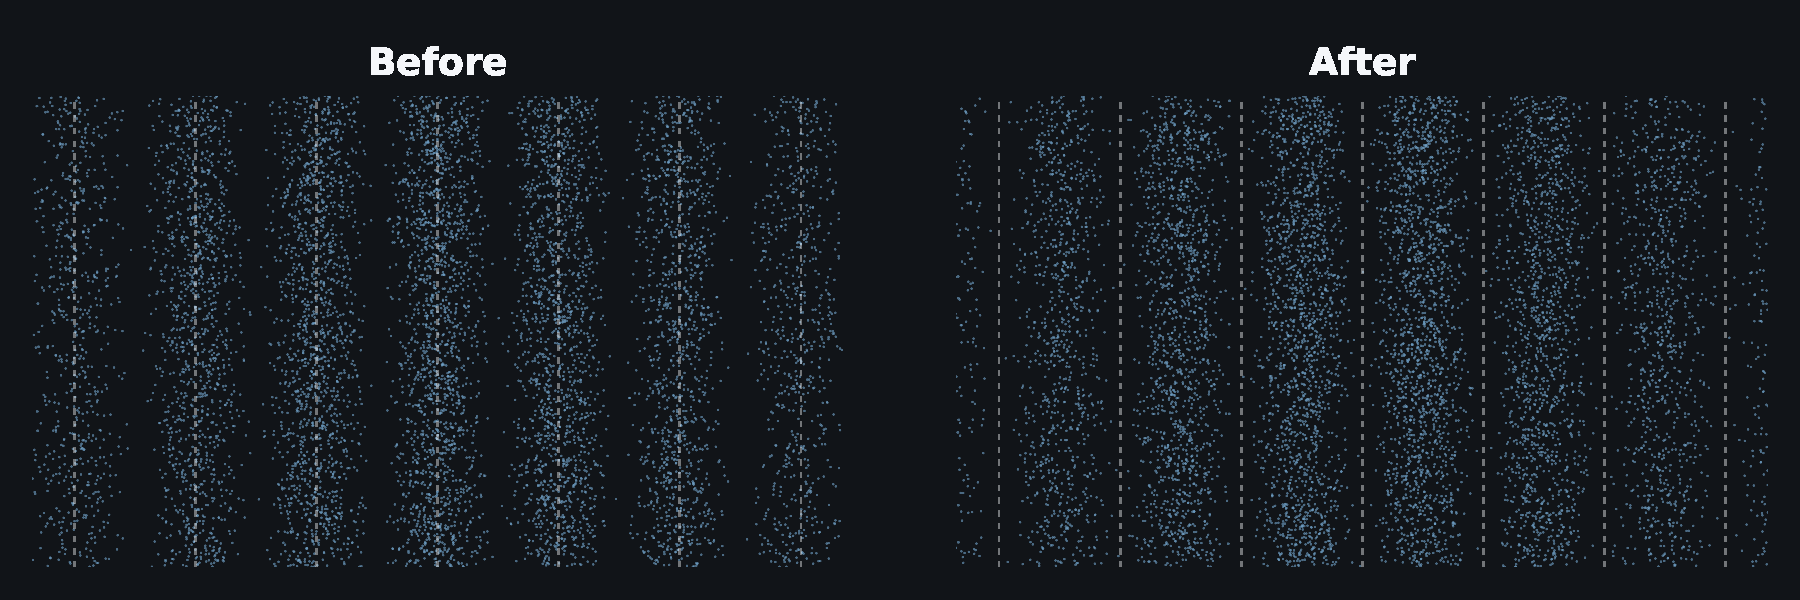
\includegraphics[width=\textwidth]{scripts/figures/interference_before_after.pdf}
	\caption{Author-generated Monte Carlo illustration of single-electron
		accumulation before and after inserting half a flux quantum,
		$\Phi_B=\Phi_0/2$. The resulting Aharonov--Bohm phase shift
		$\Delta\delta=-\pi\equiv\pi\pmod{2\pi}$ translates the fringes by half a period without changing
		the diffraction envelope. The dashed lines mark the original maxima.}
	\label{fig:ab-half-flux-shift}
\end{figure}
\vspace{-15pt}
No force is exerted on the electrons at any point of their
trajectories.

Aharonov and Bohm already observed that comparing patterns recorded with and without flux is experimentally awkward, and suggested instead varying the flux within a single exposure, so that the alteration of the fringes is recorded directly.

\section{The toroidal experiment of Tonomura}
\label{sec:tonomura}
The prediction of a fringe shift controlled by an inaccessible flux was tested
soon after the original paper, first by
Chambers~\cite{chambersShiftElectronInterference1960} and later, with a
biprism-and-solenoid geometry, by M\"ollenstedt and
Bayh~\cite{mllenstedtMessungKontinuierlichenPhasenschiebung1962}. These experiments
observed the expected displacement of the interference pattern, but they were
open to a persistent objection: no real solenoid is infinite, and a finite
solenoid leaks a small stray field into the region crossed by the electrons.
A sceptic could therefore attribute the observed shift not to the vector
potential in a field-free region, but to the electrons interacting with this
residual magnetic field along their paths.


The experiment that closed the loophole was performed by Tonomura and
collaborators in 1986 \cite{tonomuraEvidenceAharonovBohmEffect1986}. The
idea is to replace the solenoid with a geometry that has no ends from
which the field can leak, a toroid (a ring). The sample is a microscopic
toroidal magnet of permalloy, a few micrometres across, in which the magnetic
flux circulates entirely inside the ring. An electron wave is then split so
that one part passes through the hole of the toroid and
the other part passes outside it. The two partial waves enclose the magnetic
flux \(\Phi_B\) trapped in the ring, so their relative phase at recombination
is
\[
	\Delta \delta \; = \; \frac{q}{\hbar} \oint_C A \cdot dr \; = \;
	\frac{q\, \Phi_B}{\hbar},
\]
exactly as in the solenoid case, while neither wave ever travels through a
region of non-zero magnetic field.

Two further precautions make the shielding airtight. First, the toroid is
covered with a layer of niobium, a superconductor. Below its critical
temperature, a superconductor expels magnetic fields from its interior (the
Meissner effect), so the superconducting layer acts as a wall that the trapped
flux cannot cross: any residual leakage field is suppressed, not merely assumed
small. Second, the whole structure is coated with copper, which prevents the
electron wave from penetrating into the magnet itself. The electrons therefore
travel only through regions in which $B = 0$, and the flux is confined by a
physical mechanism rather than by an idealization.

The superconducting layer has a second consequence, which turns a precaution
into a signature. The magnetic flux trapped inside a superconducting ring
cannot take arbitrary values: it is quantized in integer multiples of the
superconducting flux quantum $h/2e$.\footnote{The elementary flux quantum
	associated with a charge $q$ is $\Phi_0 = h/|q|$. In a superconductor the charge
	carriers are Cooper pairs of charge $2e$, so the trapped flux is quantized in
	units of $h/2e$, half the value one would associate with a single electron.}
For an electron of charge $q = -e$, setting $\Phi_B = n\,h/2e$, with
$n\in\mathbb Z$, in the phase difference gives
\[
	\Delta\delta \;=\; -\frac{e}{\hbar}\,n\,\frac{h}{2e} \;=\; -n\pi .
\]
The predicted relative phase between the wave through the hole and the wave
outside is therefore, modulo $2\pi$, either $0$ (for even $n$) or $\pi$ (for odd $n$), and
nothing in between. A phase of $\pi$ corresponds to a displacement of the
interference fringes inside the hole by exactly half a fringe spacing with
respect to the fringes outside.

This is precisely what was observed. When the sample is cooled below the
critical temperature of niobium and imaged by electron interferometry, the
fringes crossing the hole of the toroid appear shifted by half a spacing
relative to those outside, for toroids trapping an odd number of flux quanta,
and unshifted for an even number. The interference micrographs show this
directly: the fringe system inside the hole is displaced by half a period with
respect to the reference fringes, even though the magnetic field is confined
inside the shielded ring.
\begin{figure}[H]
	\centering
	\begin{subfigure}[t]{0.48\textwidth}
		\centering
		\includegraphics[width=\linewidth]{../assets/figures/%
			tonomura_torus_unshifted.pdf}
		\caption{Below $T_c$, even $n$: no relative phase shift.}
		\label{fig:tonomura-torus-unshifted}
	\end{subfigure}
	\hfill
	\begin{subfigure}[t]{0.48\textwidth}
		\centering
		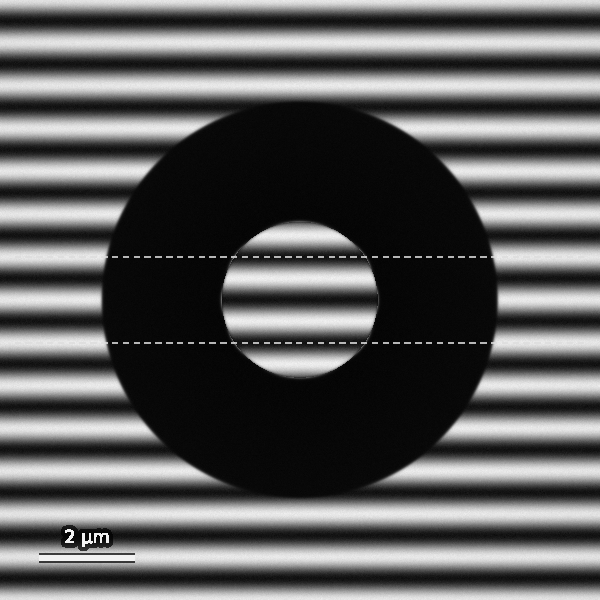
\includegraphics[width=\linewidth]{../assets/figures/tonomura_torus_shifted.pdf}
		\caption{Below $T_c$, odd $n$: $\Delta\delta\equiv\pi\pmod{2\pi}$.}
		\label{fig:tonomura-torus-shifted}
	\end{subfigure}
	\caption{Schematic comparison of even and odd trapped flux quanta below
		$T_c$. The fixed
		dashed guides mark an outside maximum: with no phase offset the same
		maximum continues through the hole, whereas the Aharonov--Bohm phase
		moves the interior pattern by half a fringe spacing. Author-generated
		schematic based on the toroidal experiment of Tonomura
		et al.~\cite{tonomuraEvidenceAharonovBohmEffect1986}.}
	\label{fig:tonomura-torus-comparison}
\end{figure}
The result leaves no room for the stray-field objection. The electrons move
exclusively in a region where $B = 0$, enforced by the Meissner effect rather
than by geometry alone, and yet their interference pattern records the enclosed
flux. What the electrons respond to is not the field along their paths, which
vanishes, but the gauge-invariant circulation $\oint_C A\cdot dr = \Phi_B$,
which does not. The Aharonov--Bohm phase is therefore a genuine physical
effect: a non-local, gauge-invariant functional of the vector potential is
observable even when the field itself is everywhere inaccessible.
